\documentclass[aspectratio=169,10pt]{beamer}
\usetheme{Madrid}
\usecolortheme{whale}
\usefonttheme{professionalfonts}

\usepackage[utf8]{inputenc}
\usepackage[T1]{fontenc}
\usepackage[brazil]{babel}
\usepackage{graphicx}
\usepackage{booktabs}
\usepackage{listings}
\usepackage{xcolor}
\usepackage{tikz}
\usetikzlibrary{arrows.meta,positioning,shapes.geometric,fit,backgrounds}
\usepackage{hyperref}

\definecolor{imeblue}{RGB}{0,43,92}
\definecolor{imegold}{RGB}{197,155,39}
\definecolor{codebg}{RGB}{245,247,250}
\definecolor{okgreen}{RGB}{27,126,50}
\definecolor{alertred}{RGB}{190,25,25}

\setbeamercolor{palette primary}{bg=imeblue,fg=white}
\setbeamercolor{palette secondary}{bg=imeblue!85!black,fg=white}
\setbeamercolor{palette tertiary}{bg=imeblue!70!black,fg=white}
\setbeamercolor{structure}{fg=imeblue}
\setbeamercolor{title}{bg=imeblue,fg=white}
\setbeamercolor{frametitle}{bg=imeblue,fg=white}
\setbeamercolor{block title}{bg=imeblue,fg=white}
\setbeamercolor{block body}{bg=codebg,fg=black}
\setbeamercolor{block title alerted}{bg=alertred,fg=white}
\setbeamercolor{block body alerted}{bg=alertred!8!white,fg=black}
\setbeamercolor{block title example}{bg=okgreen,fg=white}
\setbeamercolor{block body example}{bg=okgreen!8!white,fg=black}

\setbeamertemplate{navigation symbols}{}
\setbeamertemplate{footline}{
  \leavevmode%
  \hbox{%
  \begin{beamercolorbox}[wd=.36\paperwidth,ht=2.5ex,dp=1ex,left]{author in head/foot}%
    \hspace*{2ex}\usebeamerfont{author in head/foot}Grupo 3 --- Pariz, Mateus Roma e Daniel Coimbra
  \end{beamercolorbox}%
  \begin{beamercolorbox}[wd=.44\paperwidth,ht=2.5ex,dp=1ex,center]{title in head/foot}%
    \usebeamerfont{title in head/foot}Monitoramento Inteligente de Carga --- STM32MP157D-DK1
  \end{beamercolorbox}%
  \begin{beamercolorbox}[wd=.20\paperwidth,ht=2.5ex,dp=1ex,right]{date in head/foot}%
    \usebeamerfont{date in head/foot}\insertframenumber{} / \inserttotalframenumber\hspace*{2ex}
  \end{beamercolorbox}}%
  \vskip0pt%
}

\lstset{
  basicstyle=\ttfamily\scriptsize,
  backgroundcolor=\color{codebg},
  frame=single,
  rulecolor=\color{imeblue!30},
  breaklines=true,
  keywordstyle=\color{imeblue}\bfseries,
  commentstyle=\color{okgreen!80!black}\itshape,
  stringstyle=\color{alertred},
  showstringspaces=false
}

\title[Monitoramento de Carga --- STM32MP1]{Monitoramento Inteligente de Carga Sens\'{i}vel\\STM32MP157D-DK1 \& Linux Industrial I/O (IIO)}
\subtitle{Programa\c{c}\~{a}o Aplicada \`{a} Engenharia El\'{e}trica --- Projeto Final}
\author[Grupo 3 --- SE/3 IME]{Jo\~{a}o Victor Tavares Pariz \and Mateus Roma \and Daniel Coimbra}
\institute[IME --- SE/3]{
  Instituto Militar de Engenharia --- IME\\
  Se\c{c}\~{a}o de Engenharia El\'{e}trica --- SE/3 (Eletr\^{o}nica)
}
\date{Novembro de 2026}

\begin{document}

% ============================================================================
% SLIDE 1: CAPA
% ============================================================================
\begin{frame}
  \titlepage
  \vspace{-0.4cm}
  \begin{center}
    \scriptsize
    \textbf{Reposit\'{o}rio GitHub:} \texttt{github.com/VPariz/stm32-projeto-final-prog-aplicada}\\
    \textbf{Hardware:} Kit STMicroelectronics STM32MP157D-DK1 \quad|\quad \textbf{Sensor:} Infravermelho Reflexivo HW-201 (LM393)
  \end{center}
\end{frame}

% ============================================================================
% SLIDE 2: VISAO GERAL E LINHA DO TEMPO DE COMMITS
% ============================================================================
\begin{frame}{1. Vis\~{a}o Geral e Linha do Tempo de Commits no GitHub}
  \begin{block}{Problema Operacional e Solu\c{c}\~{a}o Embarcada}
    Monitoramento cont\'{i}nuo contra viola\c{c}\~{a}o f\'{i}sica/abertura de compartimento de carga sens\'{i}vel utilizando \textbf{C++17 estritamente Orientado a Objetos} (zero vari\'{a}veis globais) sobre o subsistema \textbf{Linux Industrial I/O (IIO)} na placa \texttt{STM32MP157D-DK1}, com telemetria UDP em tempo real e interface supervis\'{o}ria Python.
  \end{block}

  \vspace{0.1cm}
  \centering
  \footnotesize
  \begin{tabular}{llp{6.5cm}l}
    \toprule
    \textbf{Etapa} & \textbf{Prazo} & \textbf{Escopo T\'{e}cnico no Reposit\'{o}rio} & \textbf{Commit Principal} \\
    \midrule
    \textbf{Entrega 0} & 19/10/2026 & Conex\~{a}o f\'{i}sica segura com kit desligado e alimenta\c{c}\~{a}o estrita em $3{,}3\text{ V}$. & \texttt{ed3eb08} \\
    \textbf{Entrega 1} & 26/10/2026 & Classe C++ \texttt{IrObstacleSensor} encapsulada + Documenta\c{c}\~{a}o Doxygen. & \texttt{933267a} \\
    \textbf{Entrega 2} & 02/11/2026 & Cross-compila\c{c}\~{a}o ARM, leitura real via Linux IIO e deploy via SCP. & \texttt{d4b8184} \\
    \textbf{Entrega 3} & 09/11/2026 & Classe \texttt{UdpTransmitter}, envio UDP ao servidor e protocolo JSON. & \texttt{8fb8f14} $\rightarrow$ \texttt{779a547} \\
    \textbf{Entrega 4} & 16/11/2026 & Interface Gr\'{a}fica Python (hist\'{o}rico 60s, alarme, limiar e CSV) + Slides. & \texttt{Entrega Final} \\
    \bottomrule
  \end{tabular}
\end{frame}

% ============================================================================
% SLIDE 3: FLUXOGRAMA DO SISTEMA
% ============================================================================
\begin{frame}{2. Fluxograma e Arquitetura Completa do Sistema}
  \centering
  \begin{tikzpicture}[
    node distance=0.55cm and 0.65cm,
    box/.style={rectangle, rounded corners=4pt, draw=imeblue, thick, fill=codebg, align=center, font=\scriptsize, minimum height=1.05cm, text width=2.95cm},
    hw/.style={box, draw=alertred!80!black, fill=alertred!7},
    linux/.style={box, draw=imeblue, fill=imeblue!7},
    pc/.style={box, draw=okgreen!85!black, fill=okgreen!8},
    arr/.style={-{Stealth[length=2.2mm]}, thick, color=imeblue!80!black}
  ]
    \node[hw] (sensor) {\textbf{1. Sensor HW-201}\\Reflex\~{a}o IR (LM393)\\Sinal $0{,}0$ a $3{,}3\text{ V}$};
    \node[hw, right=of sensor] (adc) {\textbf{2. Hardware STM32}\\Header Analog Pino 5\\Conversor ADC 12 bits};
    \node[linux, right=of adc] (iio) {\textbf{3. Kernel Linux IIO}\\Driver \texttt{stm32-adc}\\Arquivo \texttt{in\_voltageX\_raw}};
    \node[linux, right=of iio] (cpp) {\textbf{4. App C++17 POO}\\\texttt{IrObstacleSensor}\\L\^{e}, converte e diagnostica};

    \node[linux, below=0.85cm of cpp] (udp) {\textbf{5. Socket UDP/IPv4}\\\texttt{UdpTransmitter}\\Payload JSON (Porta 5000)};
    \node[pc, left=of udp] (gui) {\textbf{6. Dashboard Python}\\\texttt{TelemetryDashboard}\\Thread UDP + Tkinter};
    \node[pc, left=of gui] (plot) {\textbf{7. Gr\'{a}fico \& Alarme}\\Janela deslizante 60 s\\Banner Verde / Vermelho};
    \node[pc, left=of plot] (csv) {\textbf{8. Persist\^{e}ncia CSV}\\Log cont\'{i}nuo em disco\\+ Exporta\c{c}\~{a}o sob demanda};

    \draw[arr] (sensor) -- (adc);
    \draw[arr] (adc) -- (iio);
    \draw[arr] (iio) -- (cpp);
    \draw[arr] (cpp) -- node[right,font=\tiny]{$250\text{ ms}$ ($4\text{ Hz}$)} (udp);
    \draw[arr] (udp) -- node[above,font=\tiny]{Ethernet} (gui);
    \draw[arr] (gui) -- (plot);
    \draw[arr] (plot) -- (csv);
  \end{tikzpicture}

  \vspace{0.35cm}
  \begin{block}{L\'{o}gica de Decis\~{a}o Embarcada em Tempo Real}
    \footnotesize
    Cada amostra ($4\text{ Hz}$) percorre o fluxo completo: \texttt{readRaw()} $\rightarrow$ $V = \frac{\text{ADC}}{4095}\cdot 3{,}3\text{ V}$ $\rightarrow$ compara\c{c}\~{a}o com limiar (\texttt{raw >= 2000}) $\rightarrow$ envio UDP JSON $\rightarrow$ atualiza\c{c}\~{a}o da curva e do alarme visual no PC.
  \end{block}
\end{frame}

% ============================================================================
% SLIDE 4: ENTREGA 0 - DESCRICAO DO SENSOR E CONEXAO FISICA
% ============================================================================
\begin{frame}{3. Descri\c{c}\~{a}o do Sensor HW-201 e Conex\~{a}o F\'{i}sica Segura (Entrega 0)}
  \begin{columns}[T,onlytextwidth]
    \begin{column}{0.48\textwidth}
      \begin{block}{Funcionamento do Sensor HW-201 (LM393)}
        \begin{itemize}
          \item Emissor e receptor infravermelho com comparador \textbf{LM393} (\textit{active-low}).
          \item \textbf{Tampa Fechada:} feixe IR reflete na tampa $\rightarrow$ sa\'{i}da baixa ($\approx 0{,}68\text{ V}$).
          \item \textbf{Tampa Aberta:} sem reflex\~{a}o $\rightarrow$ sa\'{i}da vai a n\'{i}vel alto ($\approx 2{,}90\text{ V}$).
        \end{itemize}
      \end{block}

      \vspace{0.08cm}
      \scriptsize
      \begin{tabular}{lll}
        \toprule
        \textbf{Pino} & \textbf{Header STM32MP1} & \textbf{Posi\c{c}\~{a}o} \\
        \midrule
        \textbf{VCC} ($3{,}3\text{ V}$) & Bloco Dir. (Power) & \textbf{Pino 4} (\texttt{3V3}) \\
        \textbf{GND} (Terra) & Bloco Dir. (Power) & \textbf{Pino 7} (\texttt{GND}) \\
        \textbf{OUT} (Sinal) & Bloco Esq. (Analog) & \textbf{Pino 5} (\texttt{ADC}) \\
        \bottomrule
      \end{tabular}
    \end{column}

    \begin{column}{0.49\textwidth}
      \centering
      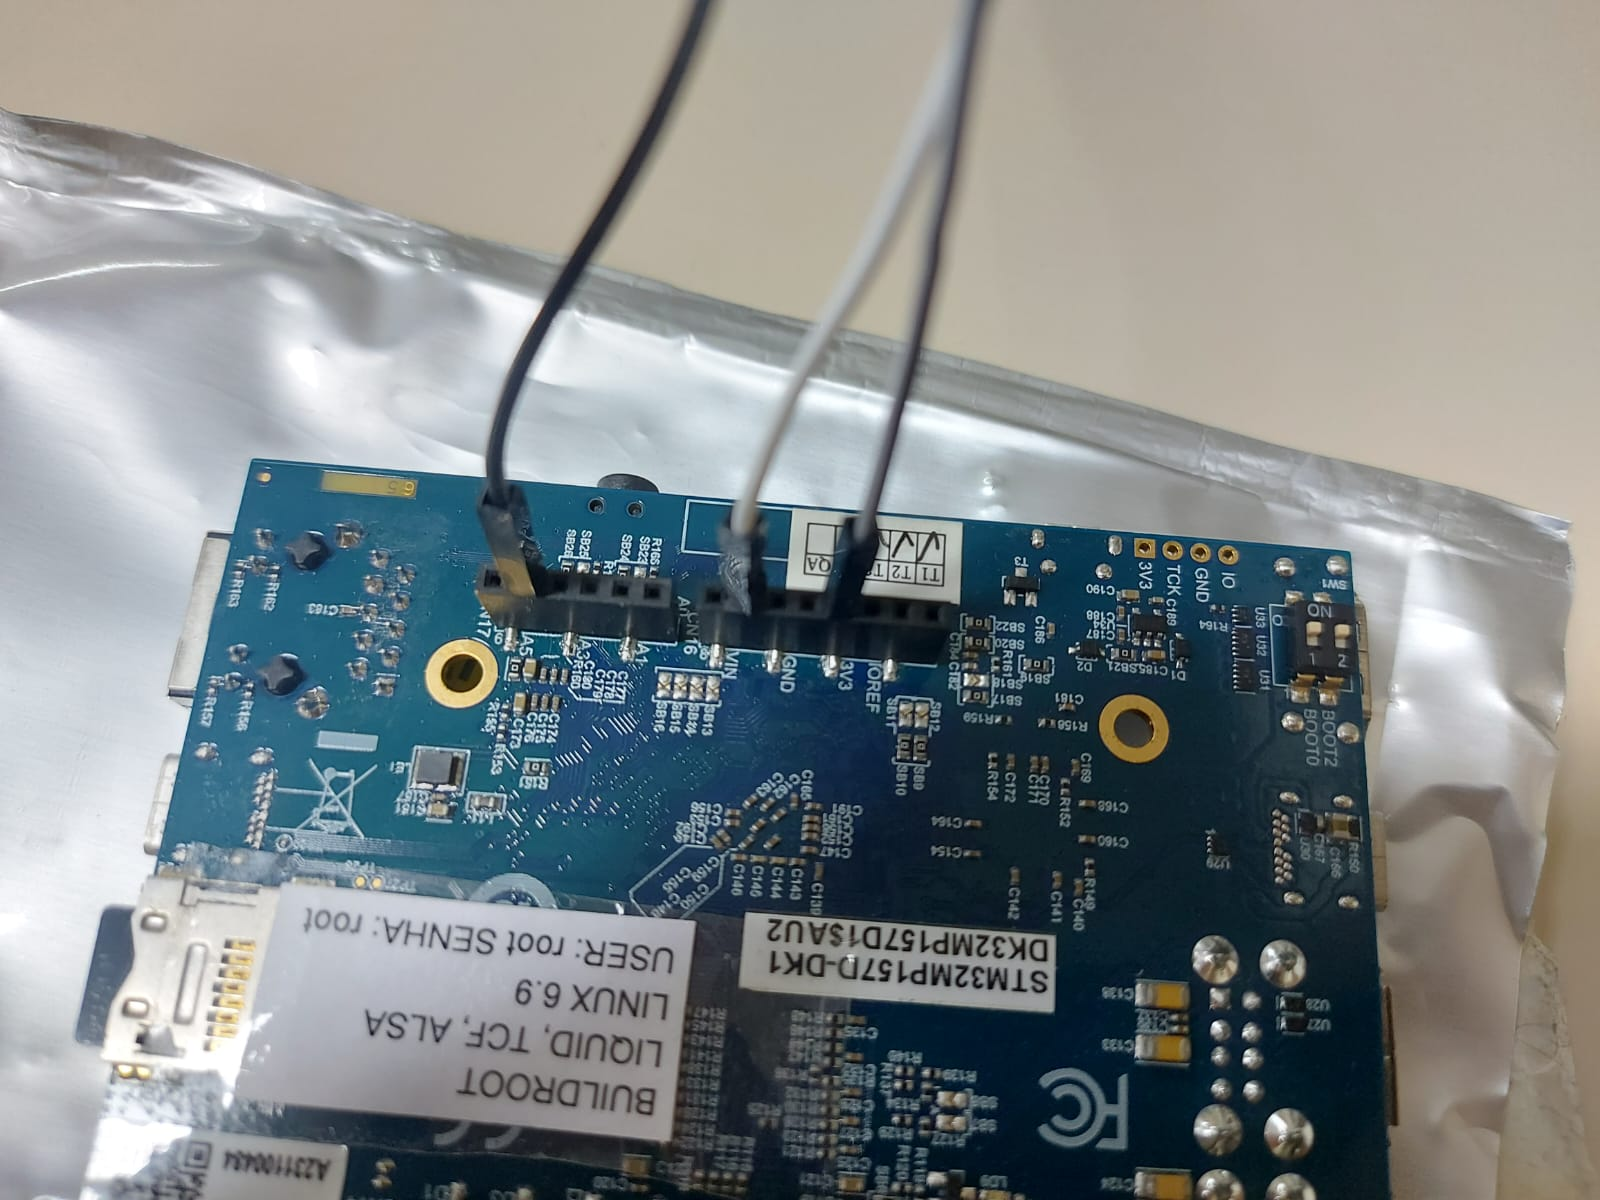
\includegraphics[width=0.47\textwidth,height=3.9cm,keepaspectratio]{../docs/conexao_placa_desligada.jpg}\hfill
      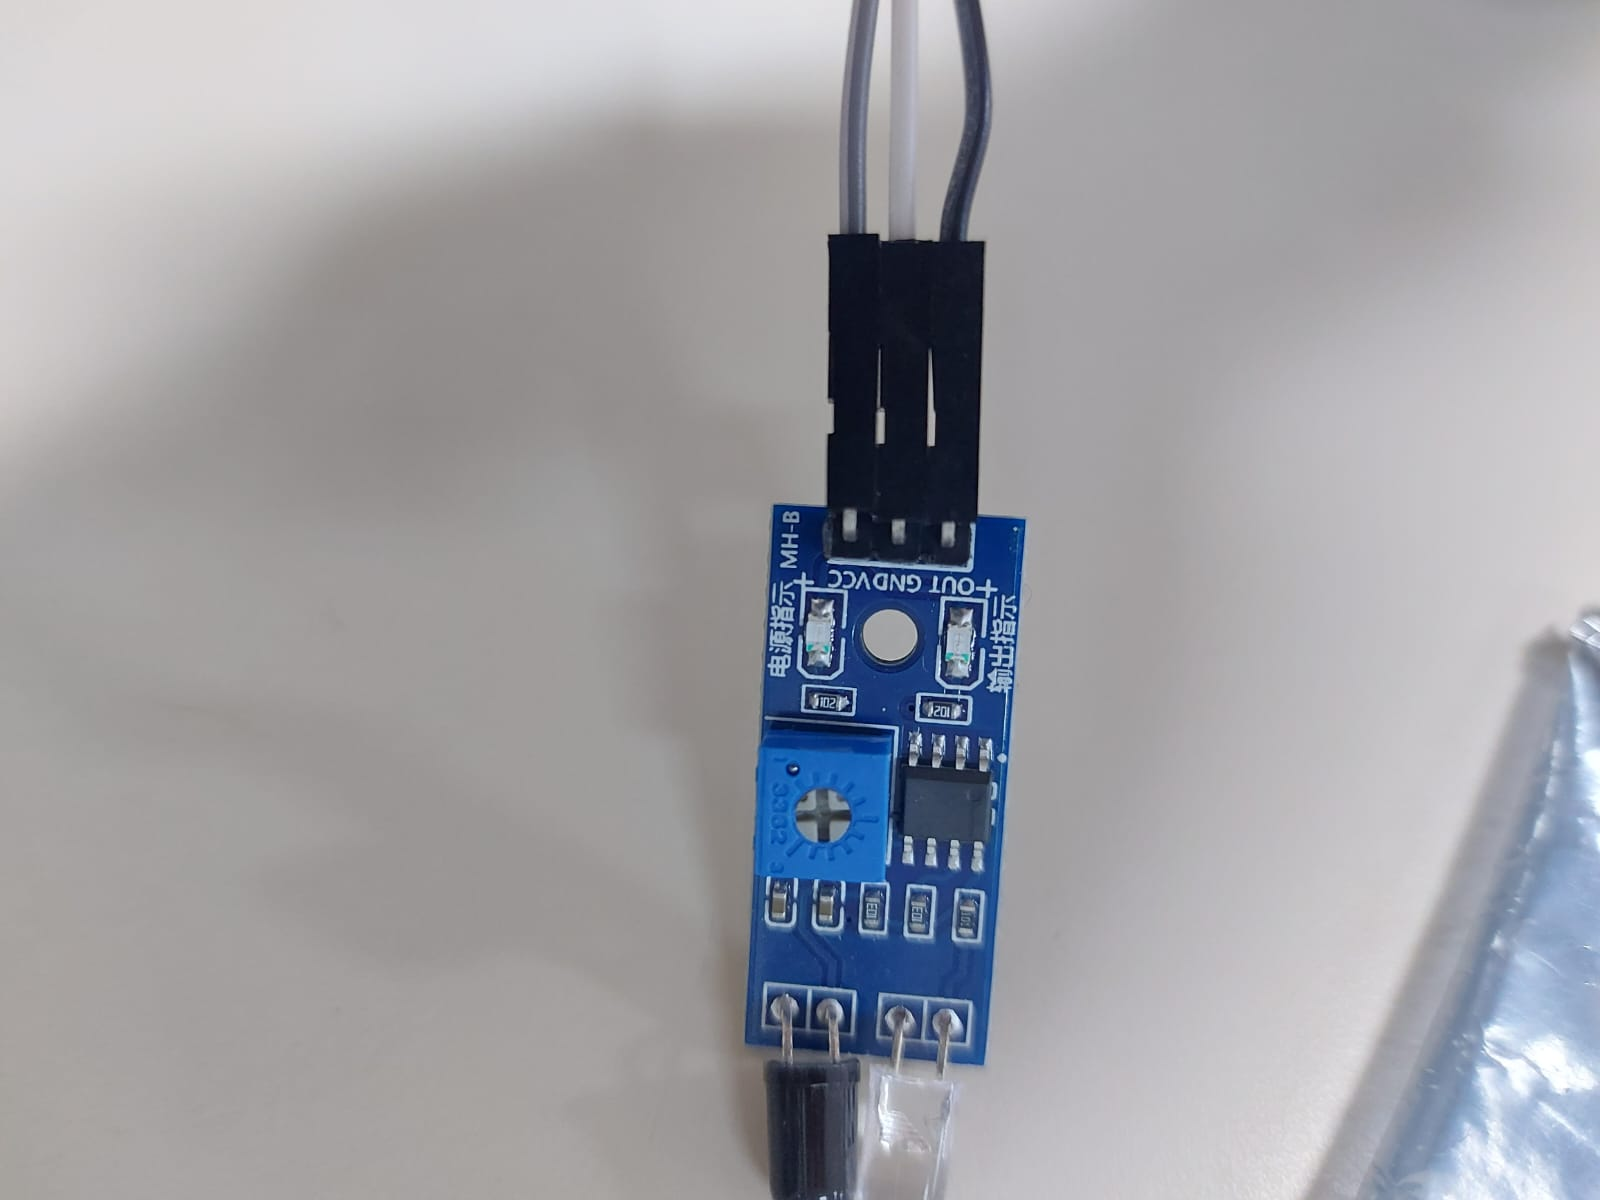
\includegraphics[width=0.47\textwidth,height=3.9cm,keepaspectratio]{../docs/conexao_sensor_pinos.jpg}
      \vspace{0.1cm}

      {\scriptsize Montagem com o kit totalmente desligado e alimenta\c{c}\~{a}o estrita em $3{,}3\text{ V}$ (\texttt{commit ed3eb08}).}
    \end{column}
  \end{columns}
\end{frame}

% ============================================================================
% SLIDE 5: DIAGRAMA DE CLASSES UML E DOXYGEN
% ============================================================================
\begin{frame}[fragile]{4. Diagrama de Classes UML, POO e Doxygen (Entregas 1 e 3)}
  \begin{columns}[T,onlytextwidth]
    \begin{column}{0.33\textwidth}
      \begin{block}{\texttt{IrObstacleSensor} (C++17)}
        \tiny
        \textbf{Privado:}
        \begin{itemize}\setlength\itemsep{1pt}
          \item \texttt{devicePath : string}
          \item \texttt{rawThreshold : int}
          \item \texttt{lastRawValue : int}
          \item \texttt{referenceVoltage : double}
          \item \texttt{maxAdcResolution : int}
          \item \texttt{autoDetectIioChannel()}
        \end{itemize}
        \textbf{P\'{u}blico:}
        \begin{itemize}\setlength\itemsep{1pt}
          \item \texttt{readRaw() : int}
          \item \texttt{getVoltage() : double}
          \item \texttt{isObstacleDetected()}
          \item \texttt{isCompartmentViolated()}
          \item \texttt{runTelemetryLoop(...)}
        \end{itemize}
      \end{block}
    \end{column}

    \begin{column}{0.33\textwidth}
      \begin{block}{\texttt{UdpTransmitter} (C++17)}
        \tiny
        \textbf{Privado:}
        \begin{itemize}\setlength\itemsep{1pt}
          \item \texttt{serverIp : string}
          \item \texttt{serverPort : int}
          \item \texttt{sensorId : string}
          \item \texttt{sockfd : SOCKET} (RAII)
          \item \texttt{initSocket() / cleanupSocket()}
        \end{itemize}
        \textbf{P\'{u}blico:}
        \begin{itemize}\setlength\itemsep{1pt}
          \item \texttt{sendRawMessage(...)}
          \item \texttt{sendTelemetryJson(...)}
          \item \texttt{sendTelemetryCsv(...)}
          \item \texttt{setServerIp() / getServerIp()}
          \item \texttt{setServerPort() / getServerPort()}
        \end{itemize}
      \end{block}
    \end{column}

    \begin{column}{0.31\textwidth}
      \begin{exampleblock}{\texttt{TelemetryDashboard} (Py)}
        \tiny
        \textbf{Atributos:}
        \begin{itemize}\setlength\itemsep{1pt}
          \item \texttt{udp\_port = 5000}
          \item \texttt{times, voltages (maxlen=240)}
          \item \texttt{threshold = 2000}
          \item \texttt{csv\_filename}
        \end{itemize}
        \textbf{M\'{e}todos:}
        \begin{itemize}\setlength\itemsep{1pt}
          \item \texttt{udp\_listener()}
          \item \texttt{update\_gui\_loop()}
          \item \texttt{on\_threshold\_change()}
          \item \texttt{export\_csv()}
        \end{itemize}
      \end{exampleblock}
    \end{column}
  \end{columns}

  \vspace{0.08cm}
  \begin{alertblock}{Boas Pr\'{a}ticas de Engenharia de Software}
    \scriptsize
    \textbf{Zero vari\'{a}veis globais}, encapsulamento estrito, compatibilidade dual POSIX/WinSock e documenta\c{c}\~{a}o HTML gerada via \texttt{doxygen Doxyfile} em \texttt{docs/doxygen/html/index.html} (\texttt{933267a}, \texttt{779a547}).
  \end{alertblock}
\end{frame}

% ============================================================================
% SLIDE 6: COMPILACAO, USO E ANALISE DOS VALORES MEDIDOS
% ============================================================================
\begin{frame}[fragile]{5. Instru\c{c}\~{o}es de Compila\c{c}\~{a}o, Uso e An\'{a}lise dos Valores Medidos}
  \begin{columns}[T,onlytextwidth]
    \begin{column}{0.48\textwidth}
      \begin{block}{Compila\c{c}\~{a}o Cruzada ARM e Execu\c{c}\~{a}o (\texttt{commit d4b8184})}
\begin{lstlisting}[language=bash]
# Compilacao nativa (PC / testes):
make clean && make

# Compilacao cruzada ARM (STM32MP1):
make cross  # ou bash scripts/cross_build.sh

# Envio via SCP e execucao no kit:
scp app_sensor_arm root@192.168.42.2:/home/root/
./app_sensor_arm \
  /sys/bus/iio/devices/iio:device0/in_voltage0_raw \
  0 192.168.42.10 5000
\end{lstlisting}
      \end{block}
    \end{column}

    \begin{column}{0.49\textwidth}
      \begin{exampleblock}{An\'{a}lise F\'{i}sica das Leituras Medidas}
        \scriptsize
        Convers\~{a}o ADC 12 bits ($0$--$4095$) para $V_{\text{ref}} = 3{,}30\text{ V}$:
        \[
          V = \frac{\text{ADC}_{\text{raw}}}{4095}\times 3{,}30\text{ V}, \qquad \text{Limiar} = 2000 \;(1{,}61\text{ V})
        \]
        \begin{tabular}{llll}
          \toprule
          \textbf{Estado} & \textbf{ADC} & \textbf{Tens\~{a}o ($V$)} & \textbf{Diagn\'{o}stico} \\
          \midrule
          Fechada & $100$--$900$ ($850$) & $0{,}08$--$0{,}75\text{ V}$ & \texttt{INTEGRA} \\
          Aberta & $3500$--$4095$ ($3600$) & $2{,}80$--$3{,}30\text{ V}$ & \texttt{VIOLACAO!} \\
          \bottomrule
        \end{tabular}
      \end{exampleblock}
      \vspace{0.08cm}
      \scriptsize
      \textbf{Sa\'{i}da real no console:}
      \texttt{[0001] Bruto: 850 (0.68 V) | Obstaculo: PRESENTE | Carga: INTEGRA}\\
      \texttt{[0004] Bruto: 3600 (2.90 V) | Obstaculo: AUSENTE | VIOLACAO DETECTADA!}
    \end{column}
  \end{columns}
\end{frame}

% ============================================================================
% SLIDE 7: PROTOCOLO UDP (ENTREGA 3)
% ============================================================================
\begin{frame}[fragile]{6. Documenta\c{c}\~{a}o do Protocolo de Telemetria UDP (Entrega 3)}
  \begin{columns}[T,onlytextwidth]
    \begin{column}{0.50\textwidth}
      \begin{block}{Evolu\c{c}\~{a}o Modular em Commits}
        \begin{itemize}
          \item \texttt{8fb8f14} --- Getters de endpoint na classe \texttt{UdpTransmitter} (socket RAII \texttt{AF\_INET / SOCK\_DGRAM}).
          \item \texttt{e11bb71} --- La\c{c}o \texttt{runTelemetryLoop()} em \texttt{IrObstacleSensor} e integra\c{c}\~{a}o em \texttt{main.cpp}.
          \item \texttt{7dad673} --- Atualiza\c{c}\~{a}o do \texttt{Makefile}, \texttt{cross\_build.sh} e pipeline GitHub Actions CI.
          \item \texttt{779a547} --- Documenta\c{c}\~{a}o do protocolo UDP e Doxygen atualizado.
        \end{itemize}
      \end{block}
    \end{column}

    \begin{column}{0.47\textwidth}
      \begin{block}{Datagrama JSON UTF-8 (Porta UDP \texttt{5000})}
\begin{lstlisting}
{
  "sensor_id": "G3_IR_HW201",
  "raw": 850,
  "voltage": 0.68,
  "unit": "V",
  "violated": 0,
  "timestamp": 1762640400125
}
\end{lstlisting}
      \end{block}
      \scriptsize
      \begin{tabular}{lll}
        \toprule
        \textbf{Campo} & \textbf{Tipo} & \textbf{Significado} \\
        \midrule
        \texttt{raw} & \texttt{int} & Leitura ADC ($0$ a $4095$) \\
        \texttt{voltage} & \texttt{double} & Tens\~{a}o em Volts ($0{,}00$--$3{,}30$) \\
        \texttt{violated} & \texttt{int} & $0=$ \'{I}ntegra, $1=$ Violada \\
        \texttt{timestamp} & \texttt{int64} & \'{E}poca UNIX (ms) \\
        \bottomrule
      \end{tabular}
    \end{column}
  \end{columns}
\end{frame}

% ============================================================================
% SLIDE 8: CAPTURAS DE TELA DA INTERFACE GRAFICA (ENTREGA 4)
% ============================================================================
\begin{frame}{7. Capturas de Tela da Interface Gr\'{a}fica Supervis\'{o}ria (Entrega 4)}
  \begin{columns}[T,onlytextwidth]
    \begin{column}{0.49\textwidth}
      \centering
      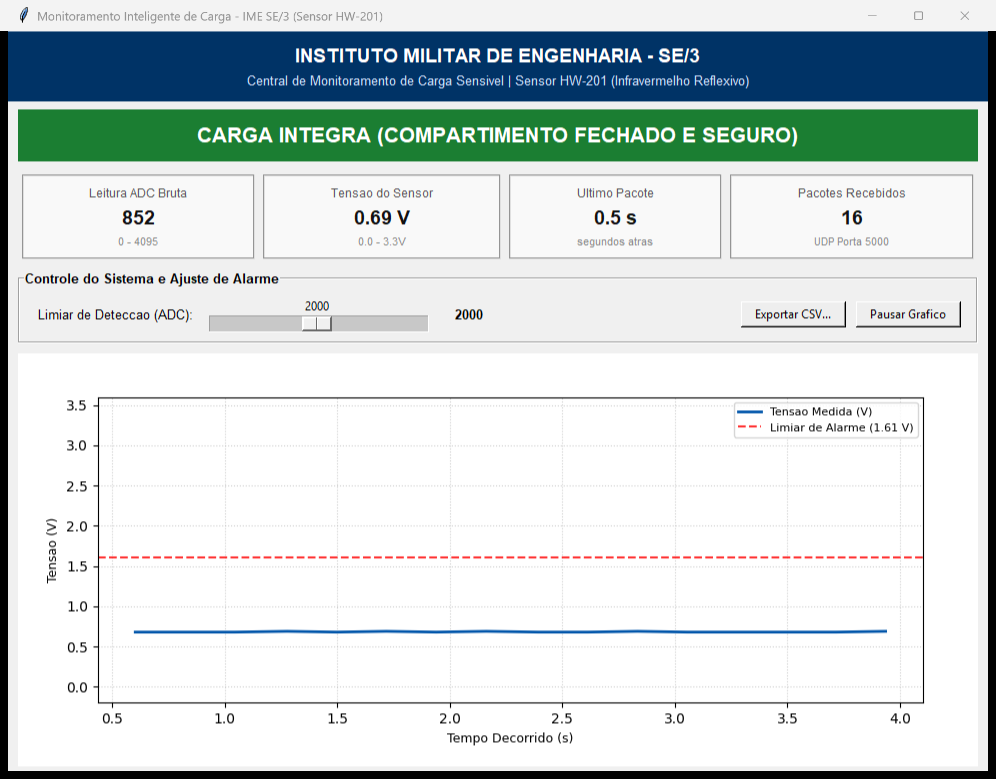
\includegraphics[width=\textwidth,height=4.3cm,keepaspectratio]{../docs/gui_carga_integra.png}
      \vspace{0.05cm}

      \scriptsize\textbf{Estado Normal:} ADC = \texttt{852} ($0{,}69\text{ V} < 1{,}61\text{ V}$) $\rightarrow$ Banner \textcolor{okgreen}{\textbf{VERDE}}.
    \end{column}

    \begin{column}{0.49\textwidth}
      \centering
      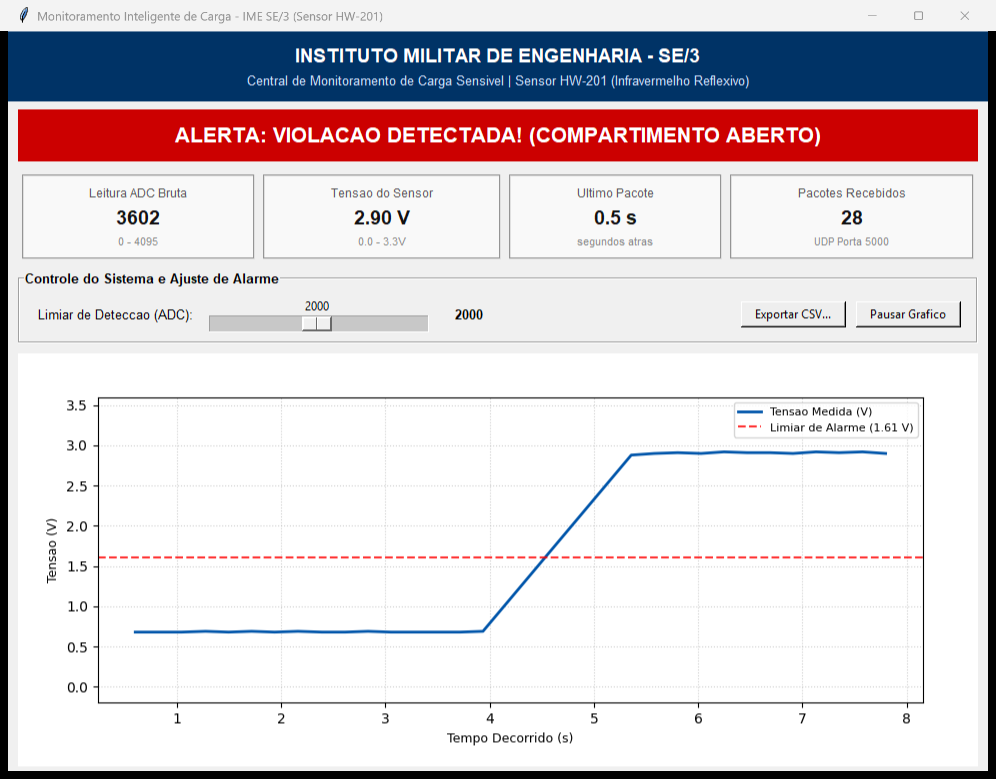
\includegraphics[width=\textwidth,height=4.3cm,keepaspectratio]{../docs/gui_alerta_violacao.png}
      \vspace{0.05cm}

      \scriptsize\textbf{Viola\c{c}\~{a}o:} ADC = \texttt{3602} ($2{,}90\text{ V} \ge 1{,}61\text{ V}$) $\rightarrow$ Banner \textcolor{alertred}{\textbf{VERMELHO}}.
    \end{column}
  \end{columns}

  \vspace{0.1cm}
  \begin{block}{Recursos Implementados em \texttt{gui/gui\_dashboard.py}}
    \scriptsize
    Janela deslizante de \textbf{60 s} ($240$ amostras a $4\text{ Hz}$), slider de \textbf{limiar din\^{a}mico}, indicador de \textbf{\'{u}ltimo pacote recebido} e log cont\'{i}nuo + exporta\c{c}\~{a}o em \textbf{CSV}.
  \end{block}
\end{frame}

% ============================================================================
% SLIDE 9: DEMONSTRACAO AO VIVO E VIDEO
% ============================================================================
\begin{frame}[fragile]{8. V\'{i}deo de Valida\c{c}\~{a}o no Hardware e Demonstra\c{c}\~{a}o ao Vivo}
  \begin{block}{Arquitetura em Execu\c{c}\~{a}o na Demonstra\c{c}\~{a}o}
    \centering
    \textbf{Aplicativo C++17 (\texttt{IrObstacleSensor} + \texttt{UdpTransmitter})}
    $\xrightarrow{\text{JSON via Socket UDP (Porta 5000)}}$
    \textbf{Dashboard Python (\texttt{TelemetryDashboard})}
  \end{block}

  \vspace{0.1cm}
  \begin{columns}[T,onlytextwidth]
    \begin{column}{0.52\textwidth}
\begin{lstlisting}[language=bash]
# 1. Iniciar a Central Grafica (Servidor UDP 5000):
python gui/gui_dashboard.py

# 2. Iniciar o Transmissor C++17 (Placa ou Local):
./app_sensor mock_sensor_raw.txt 0 127.0.0.1 5000

# (Ou via 1 clique no Windows):
apresentacao\iniciar_demo_ao_vivo.bat
\end{lstlisting}
    \end{column}

    \begin{column}{0.45\textwidth}
      \begin{exampleblock}{Checklist da Apresenta\c{c}\~{a}o}
        \begin{enumerate}
          \item V\'{i}deo do sensor HW-201 operando na placa STM32MP157D-DK1.
          \item Recebimento de pacotes UDP ao vivo ($4\text{ Hz}$) na GUI.
          \item Salto de tens\~{a}o no gr\'{a}fico + alarme vermelho.
          \item Ajuste din\^{a}mico do limiar e exporta\c{c}\~{a}o \texttt{.csv}.
        \end{enumerate}
      \end{exampleblock}
    \end{column}
  \end{columns}
\end{frame}

\end{document}
